\documentclass[12pt]{article}

\usepackage[top=1in, bottom=1in, left=1in, right=1in]{geometry} % see geometry.pdf on 
\usepackage{graphicx}
\usepackage{amssymb,amsmath}
\usepackage[utf8]{inputenc}
\usepackage{listings}
\usepackage{color}
\geometry{letterpaper}
\linespread{1.1}% \geometry{landscape} % rotated page geometry

\definecolor{codegreen}{rgb}{0,0.6,0}
\definecolor{codegray}{rgb}{0.5,0.5,0.5}
\definecolor{codepurple}{rgb}{0.58,0,0.82}
\definecolor{backcolour}{rgb}{0.95,0.95,0.92}

\lstdefinestyle{mystyle}{
	backgroundcolor=\color{backcolour},   
	commentstyle=\color{codegreen},
	keywordstyle=\color{magenta},
	numberstyle=\tiny\color{codegray},
	stringstyle=\color{codepurple},
	basicstyle=\footnotesize,
	breakatwhitespace=false,         
	breaklines=true,                 
	captionpos=b,                    
	keepspaces=true,                 
	numbers=left,                    
	numbersep=5pt,                  
	showspaces=false,                
	showstringspaces=false,
	showtabs=false,                  
	tabsize=2
}

\lstset{style=mystyle}
  
\title{IEOR 160 Course Project}
\date{20 Oct. 2017} 
\author{Qingan Zhao \\ SID: 3033030808}

\begin{document}

\maketitle
\newcommand{\ud}{\mathrm d} %COMMENT: for infinitesimal dx = \ud x and dy = \ud y TODO: DO YOURSELF all replacement
\renewcommand\theequation{\arabic{equation}}
\renewcommand{\figurename}{Fig.}
\renewcommand\thesection{Problem \arabic{section}}
\renewcommand\thesubsection{\alph{subsection} )}

\begin{large}
\noindent\textbf{All plots and relevant code are generated in MATLAB.}
\end{large}

\section{}

This problem is solved using Gradient method with the backtracking line search ($\alpha$ = 1 and $\beta$ = 0.6).\\

\noindent Code:

\lstinputlisting[language=MATLAB]{P1.m}

\bigskip\noindent The minimum value of the function is \textbf{2.722814}, where $x$=\textbf{(0.122218, -0.556434)}.\\

\noindent The plot of $f(x^{(k)})$ versus $k$ for $k=0,1,2,...,50$ is shown in Figure 1.\\\\\\

\begin{figure}[!htbp]
	\centering
	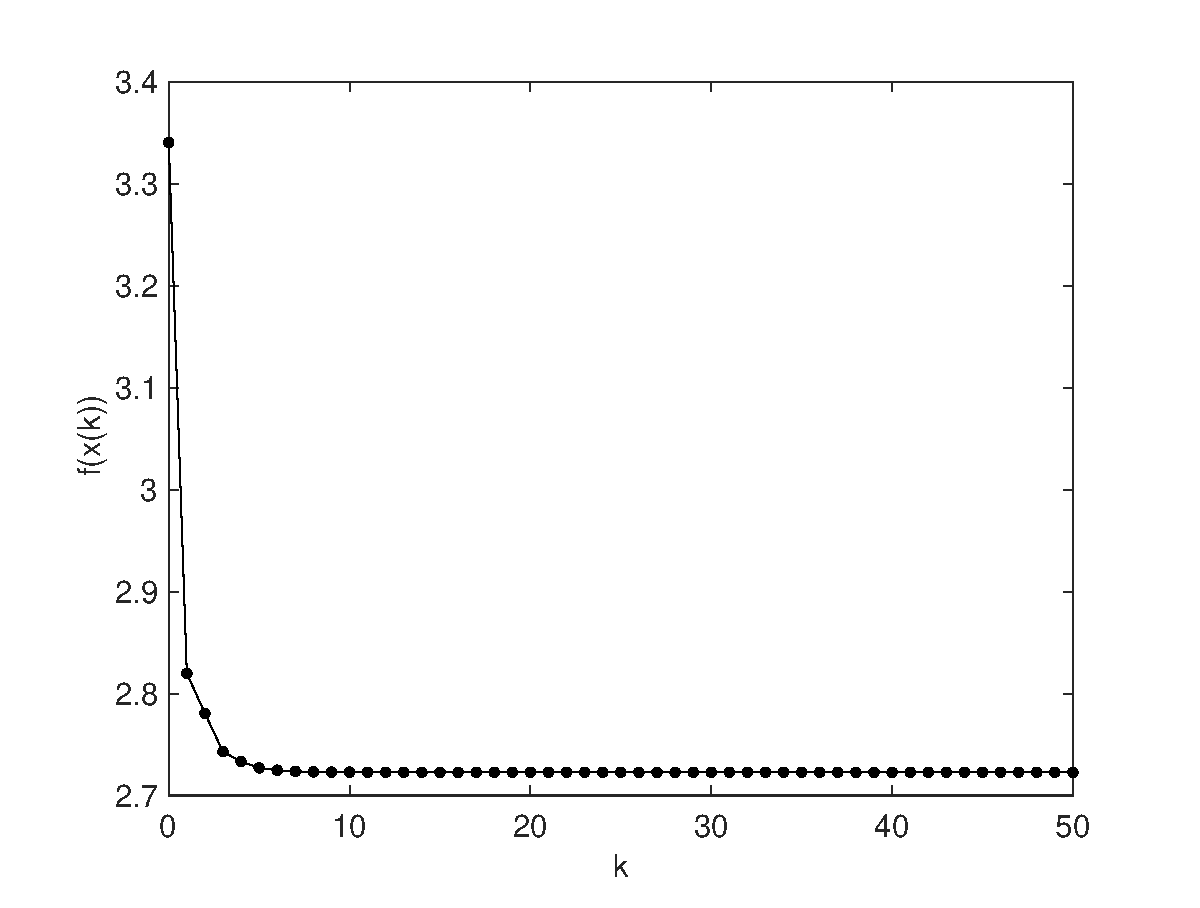
\includegraphics[width=10cm]{figures/fig1.eps}      
	\caption{$f(x^{(k)})$ versus $k$ for $k=0,1,2,...,50$ (Gradient method)}
\end{figure}

\noindent The trajectory of points $x^{(0)}$, $x^{(1)}$, ..., $x^{(50)}$ is shown in Figure 2.

\begin{figure}[!htbp]
	\centering
	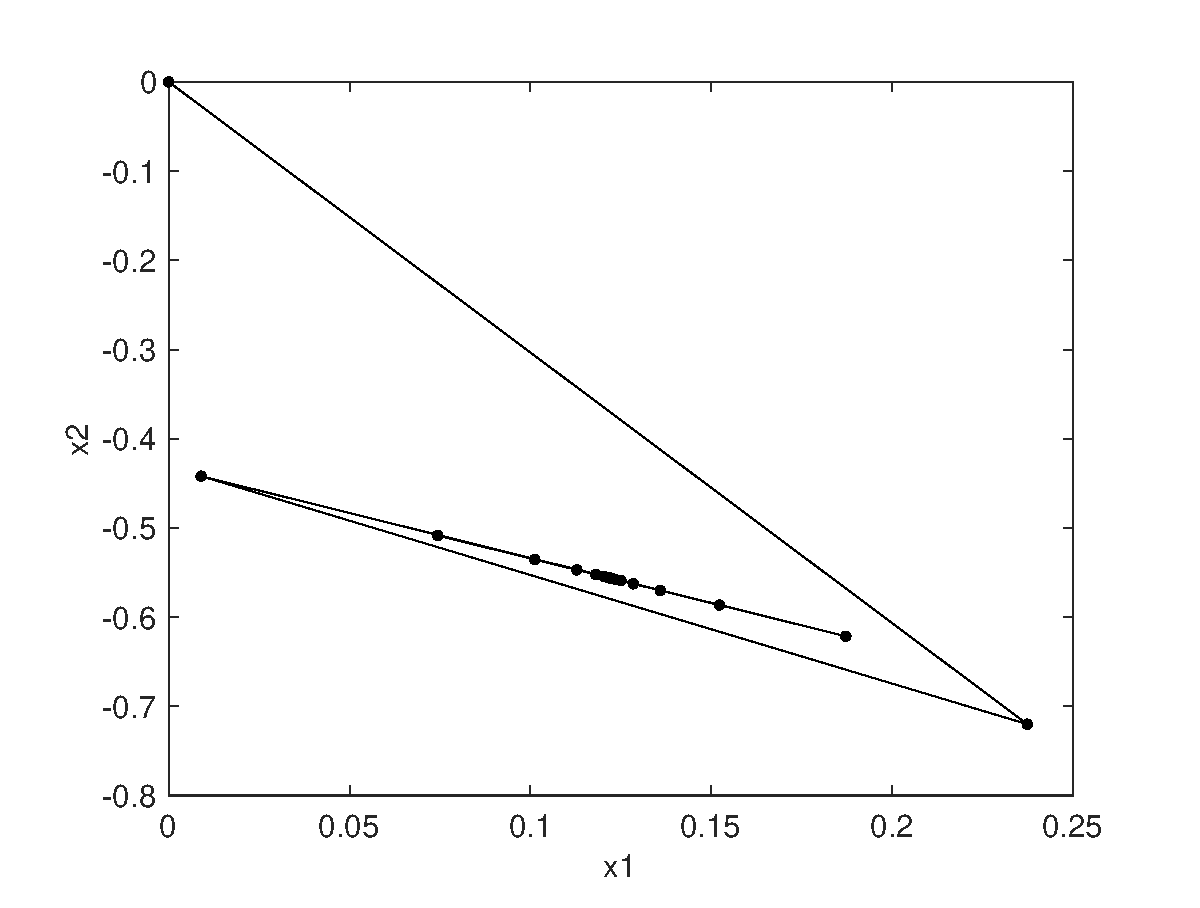
\includegraphics[width=10cm]{figures/fig2.eps}      
	\caption{The trajectory of points $x^{(0)}$, $x^{(1)}$, ..., $x^{(50)}$ (Gradient method)}
\end{figure}

\section{}

This problem is solved using Newton's method with the backtracking line search ($\alpha$ = 1 and $\beta$ = 0.6).\\

\noindent Code:

\lstinputlisting[language=MATLAB]{P2.m}

\bigskip\noindent The minimum value of the function is \textbf{2.722814}, where $x$=\textbf{(0.122219, -0.556434)}.\\

\noindent The plot of $f(x^{(k)})$ versus $k$ for $k=0,1,2,...,50$ is shown in Figure 3.

\begin{figure}[!htbp]
	\centering
	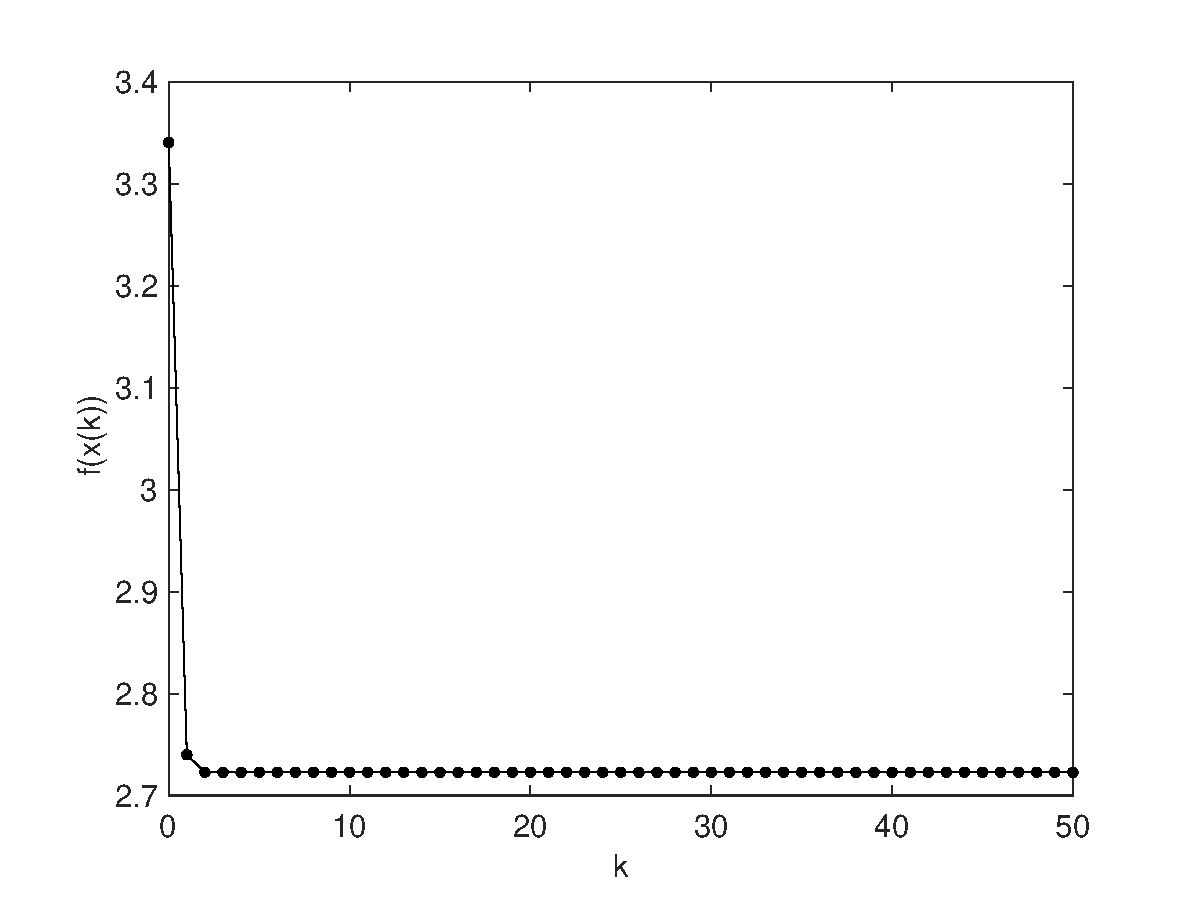
\includegraphics[width=10cm]{figures/fig3.eps}      
	\caption{$f(x^{(k)})$ versus $k$ for $k=0,1,2,...,50$ (Newton's method)}
\end{figure}

\noindent The trajectory of points $x^{(0)}$, $x^{(1)}$, ..., $x^{(50)}$ is shown in Figure 4.

\begin{figure}[!htbp]
	\centering
	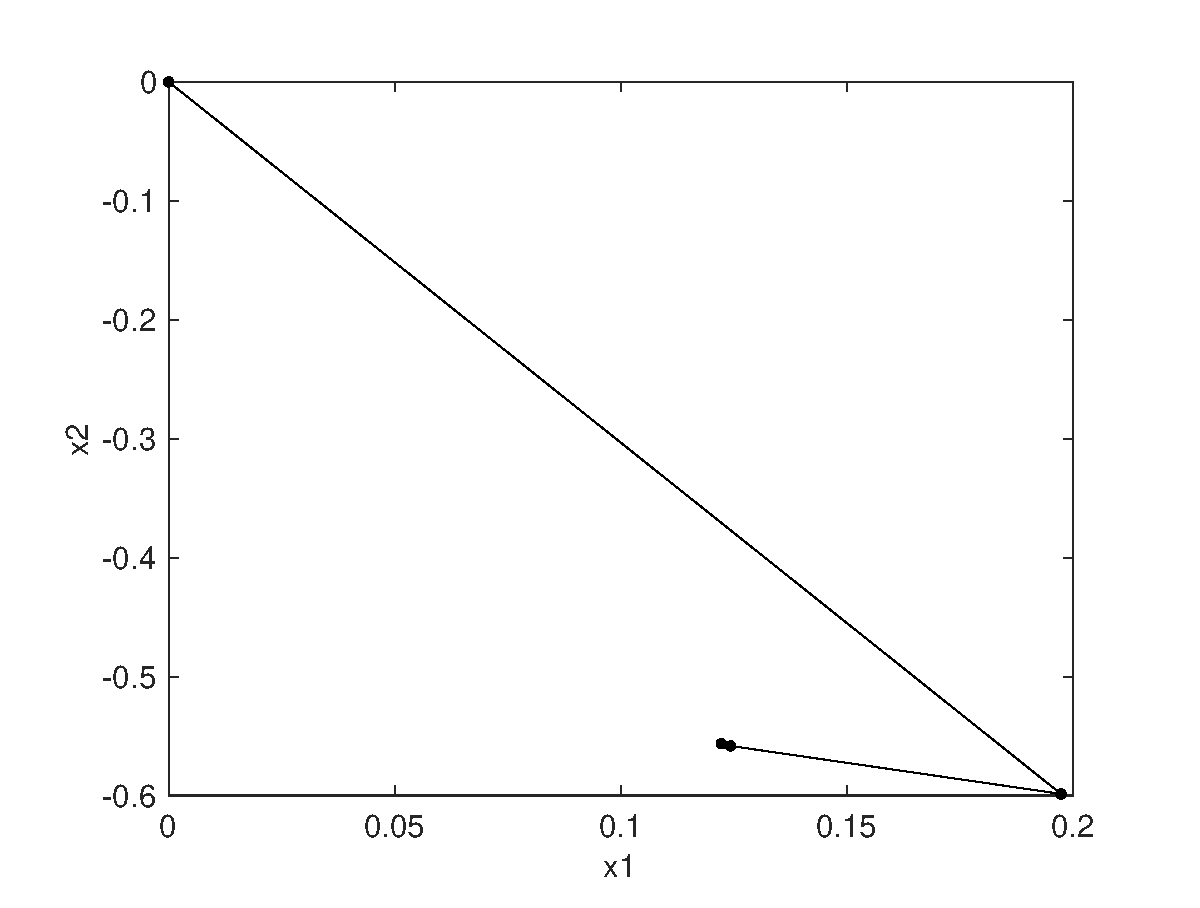
\includegraphics[width=10cm]{figures/fig4.eps}      
	\caption{The trajectory of points $x^{(0)}$, $x^{(1)}$, ..., $x^{(50)}$ (Newton's method)}
\end{figure}

\section{}

This problem is solved using Newton's method with the backtracking line search ($\alpha$ = 0.4 and $\beta$ = 0.4).\\

\noindent The function in this problem is much more complex than the previous one. Hence, to speed up the code, let's first calculate the gradient and hessian by hand instead of using $gradient()$ and $hessian()$ functions in MATLAB. Assume the $log()$ in the problem is the logarithm to the base 10.\\

\noindent Another thing needs to mention is that the code is not efficient enough to run with 500 variables, so let's just run with 100 variables instead.\\

\noindent Code:\\

\noindent\textbf{(1)} The $f$ function (the function in the problem)

\lstinputlisting[language=MATLAB]{f.m}
\ \\

\bigskip\noindent\textbf{(2)}  The gradient function

\lstinputlisting[language=MATLAB]{grad_fun.m}

\bigskip\noindent\textbf{(3)}  The hessian function

\lstinputlisting[language=MATLAB]{hess_fun.m}

\bigskip\noindent\textbf{(4)}  Main script

\lstinputlisting[language=MATLAB]{p3.m}

\bigskip\noindent The minimum value of the function is \textbf{-204.012227.}\\\\\\

\noindent The plot of $f(x^{(k)})$ versus $k$ for $k=0,1,2,...,300$ is shown in Figure 5.

\begin{figure}[!htbp]
	\centering
	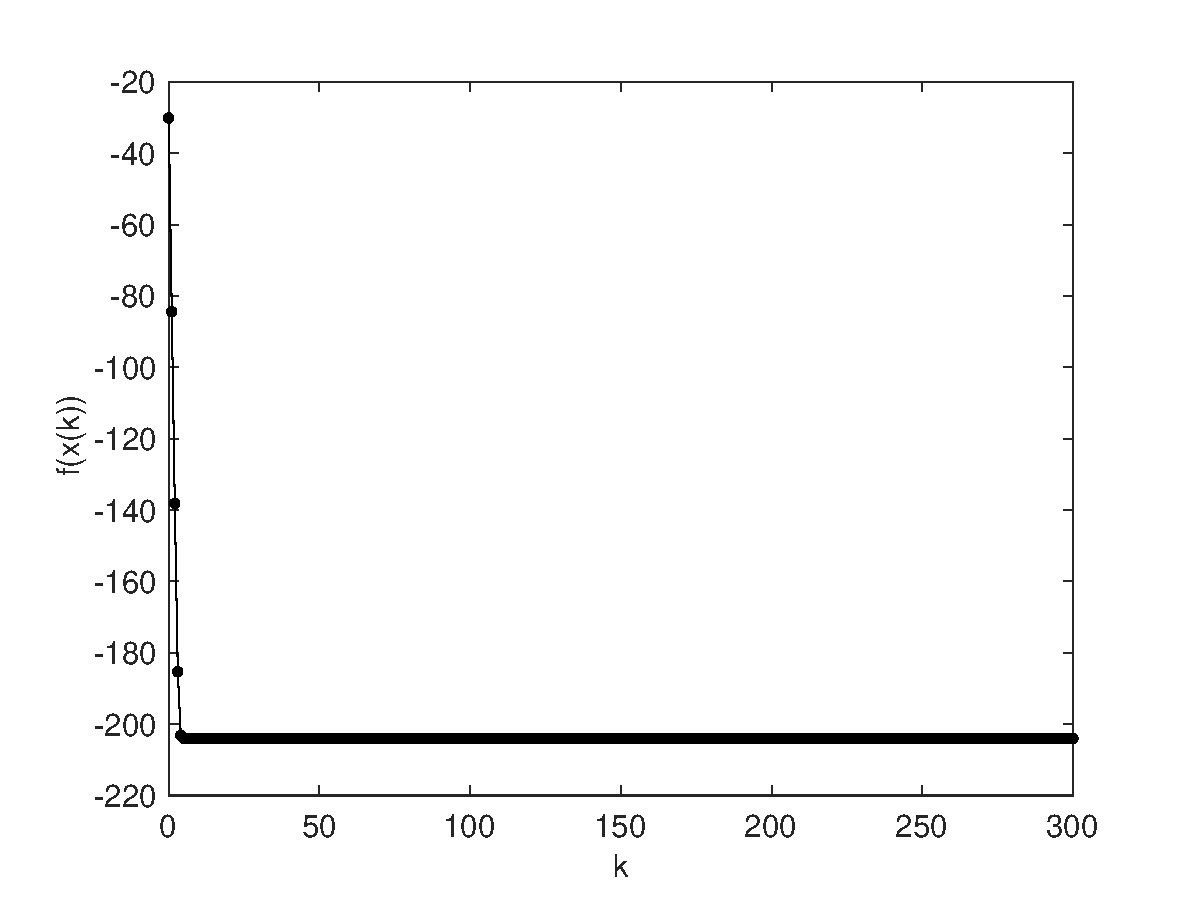
\includegraphics[width=10cm]{figures/fig5.eps}      
	\caption{$f(x^{(k)})$ versus $k$ for $k=0,1,2,...,300$ (Newton's method)}
\end{figure}

\end{document}

